\chapter{Dynamical Berry's phase and non-linear response} 
\label{chapterberry}
\section{Why do we need Berry's phase?}
%In this work we use dynamical Berry's phase to calculate the non-linear response in extended systems. 
This section presents a simple introduction to the problem of polarisation definition in extended systems and how it can be solved by means of Berry's phase concept.
\begin{wrapfigure}{r}{0.5\textwidth}
  \begin{center}
    
\includegraphics[width=0.4\textwidth]{Figures/wrong_polarization2}
  \end{center}
  \caption{Surface contribution to the polarisation in a solid. \label{surfacepol}}
\end{wrapfigure}
For many years an unsolved problem in solid state physics was the correct definition of polarisation in periodic systems.
This definition is intrinsically related to the one the dipole operator, that is a problematic object for extended systems.
In the literature different wrong definitions of bulk polarisation have been proposed that we will not cite here\cite{restanotes}.
In order to understand the problem, let's start the discussion from the polarisation in isolated systems.
In a system with open boundary conditions, the dipole operator is well defined and therefore one can write down the polarisation as:
\be
\PP = \frac{e \langle \vec \rr \rangle}{V} = \frac{e}{V}\int \vec \rr n (\rr) d \rr,
\label{polisolated}
\ee
where $n(\rr)$ is the electronic density.
The simplest idea for the definition of the polarization in periodic systems would be to generalise the previous formula. The integral in Eq.~\ref{polisolated} can be redefined in different possible ways in periodic systems. We can average the dipole operator on the whole material or consider its unit cell. In the first case we obtain $ \PP = \langle \vec \rr \rangle_{sample}/V_{sample}$. In an insulator the contributions from the dipoles inside the material cancel each other (as one can see from  Fig.~\ref{immerse}) and only the surfaces contribute to the total polarisation (see Fig.~\ref{surfacepol}):                              
\be
\Delta \PP = \frac{(\Delta \sigma L^2) L }{L ^3},
\label{polsurface}
\ee
where $\Delta \sigma$ is related to the charges accumulated on the surfaces.\cite{vanderbilt1993electric} 
This definition [Eq.~\ref{polsurface}] is not suitable for numerical calculations because it requires the simulation of the entire sample and moreover the above defined polarisation is not a bulk property but it depends from the surfaces.\\ 
The second possibility is to define the polarisation as  $ \PP = \langle \vec \rr \rangle_{cell}/V_{cell}$. But this definition is completely arbitrary. In fact different choices of the unit cell give completely different polarisations for the same material, see Fig.~\ref{cellpol}. A last possibility exists, the use of the dipole matrix elements in terms of Bloch orbitals, but also in this case there is problem since the dipole operator is unbounded in periodic systems.\\
\begin{wrapfigure}{l}{0.5\textwidth}
    \vspace{-0.7cm}
  \begin{center}
    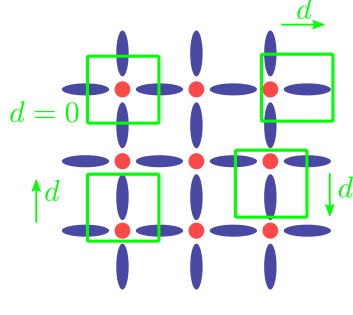
\includegraphics[width=0.4\textwidth]{Figures/wrong_polarization1}
  \end{center}
  \caption{Polarisation vector versus the choice of the unit cell. \label{cellpol} }
\end{wrapfigure}
Finally let mention that also the well know Clausius-Mossotti formula for the polarisability\cite{Mossotti} cannot be used in real solids because wave-functions are not localised objects.\\
Two reasons make polarisation definition so difficult in solids. First the dipole operator is ill defined in periodic systems, because $\vec \rr$ is not periodic while wave-functions are. Second, differently from finite systems, the polarisation cannot be expressed as an integral on the charge density\cite{Martin1998}.
This second aspect can be better understood if we write down the general relation between polarisation and density:
\be
\nabla \cdot \PP(\rr) = - n(\rr).
\ee                              
In finite systems we impose the condition  $\PP(\rr) \rightarrow 0 $ outside the sample (Dirichlet boundary condition) and $\int n(\rr) d\rr=0$.
In periodic system, it is most useful to resolve the previous equation into Fourier components $\qq+ \GG$,
where $\GG$ denotes a reciprocal lattice vector and $\qq$ belongs to the first Brillouin zone(BZ):
\be
(\qq + \GG) \cdot \PP(\qq + \GG) = i n (\qq + \GG).
\label{poldens}
\ee
It follows from Eq.~\ref{poldens} that each Fourier component can be treated separately. Now let us consider the limit $\GG=0$ and $\qq \rightarrow 0$. In this limit  the macroscopic polarisation $\PP$ is not determined anymore by the zero Fourier component of the density, which must vanish by charge neutrality.  Thus in the limit $\qq = 0$ for an infinite crystal, the polarisation contains additional information not included in the density.\cite{Martin1998} \\
The problem of a correct definition of polarisation in periodic systems was solved in 1993 by  King-Smith and Vanderbilt.\cite{KSV1} In their seminal paper they shown that  bulk polarisation can be expressed as a closed integral on the wave-function phase in the Brillouin zone, a particular case of the Berry's phase. Their formulation solved all problems with the previous attempts to define the polarisation. In fact the King-Smith and Vanderbilt(KSV) polarisation is a bulk quantity, its time derivative gives the current and its derivatives respect to the external field reproduce the polarisabilities at all orders.\\
\section{General introduction}
\emph{Ab-initio} approaches based on Green's function theory became a standard tool for quantitative and predictive calculations of linear response optical properties in Condensed Matter. In particular, the state-of-the-art approach combines the $G_0W_0$ approximation for the quasi-particle band structure~\cite{aryasetiawan1998gw} with the Bethe-Salpeter equation in static ladder approximation for the response function.~\cite{strinati} This approach proved to effectively and accurately account for the essential effects beyond independent particle approximation (IPA) in a wide range of electronic systems, including extended systems with strong excitonic effects.~\cite{Onida}

In contrast, for nonlinear optics \ai calculations of extended systems rely in large part on the IPA\cite{PhysRevB.48.11705} with correlation effects entering at most as a rigid shift of the conduction energy levels\cite{PhysRevB.80.155205}.  Within time-dependent density-functional theory (TDDFT), it has been recently proposed~\cite{PhysRevB.82.235201} an approach to calculate the second-harmonic generation (SHG) in semiconductors that takes into account as well crystal local-field and excitonic effects. However, this promising approach~\cite{Cazzanelli2012} is limited by the treatment of the electron correlation to systems with weakly bound excitons.~\cite{LRC} 

%In fact, it is extremely involved to include many-body effects into the expression for the nonlinear optical susceptibilities within Green's function theory. 
%In fact, the inclusion of many-body effects in the equations for the non-linear susceptibilities makes them very difficult to solve.
Within Green's function theory the inclusion of many-body effects into the expression for the nonlinear optical susceptibilities is extremely difficult. 
Furthermore the complexity of these expressions grows with the perturbation order. Therefore it is not surprising that there have been only few isolated attempts to calculate second-order optical susceptibility using the Bethe-Salpeter equation~\cite{Leitsmann2005,Chang2002} and no attempt to calculate higher-order optical susceptibilities.~\cite{PhysRevB.80.165318} 
%The complexity growing with the perturbation order, there have been only few isolated attempts at calculating second-order optical susceptibility using the Bethe-Salpeter equation,~\cite{Leitsmann2005,Chang2002} and in practice third-order optical susceptibility is untreatable.~\cite{PhysRevB.80.165318} 
%On the other hand, the origin of this limitation is the attempting to calculate the nonlinear optical susceptibility directly in terms of the electronic structure. 

Alternatively to the frequency-domain response-based approach, one can obtain the nonlinear optical susceptibility in time-domain from the dynamical polarisation $\PP$ of the system by using the expansion of $\PP$ in power of the applied field
\be
\label{eq:peopbf}
\PP= \chi^{(1)} \efield + \chi^{(2)} \efield^2 + \chi^{(3)} \efield^3 + \dots 
\ee 
This strategy is followed in several real-time implementations of TD-DFT\cite{PhysRevB.54.4484}. In these approaches the dynamical polarisation is obtained by numerical integration of the equations of motion (EOMs) for the Kohn-Sham system.\cite{takimoto:154114,castro:3425,meng:054110} So far applications regard mostly nonlinear optical properties in molecules.  

 
The time-domain approach presents three major advantages with respect to frequency-domain response-based approaches. First, many-body effects are included easily by adding the corresponding operator to the effective Hamiltonian. Second, it is not perturbative in the external fields and therefore it treats optical susceptibilities at any order without increasing the computational cost and with the only limitation dictated by the machine precision. Third, several non-linear phenomena and thus spectroscopic techniques are described by the same EOMs. For instance, by the superposition of several laser fields one can simulate sum- and difference-frequency harmonic generation, or four-waves mixing.\cite{boyd}

%In a recent work,~\cite{attaccalite} we proposed a real-time implementation of the Bethe-Salpeter equation, based on nonequilibrium Green's function formalism.
Although this approach shows very promising results for molecular systems, its extention to periodic system remains still limited.
In fact, due to the problems in defining the position operator and thus $\PP$, it is not trivial to apply Eq.~\eqref{eq:peopbf} to systems in which periodic boundary conditions (PBC) are imposed. As it was recognised for example in Ref.~\cite{PhysRevB.52.14636}, the same problem appears in the direct evaluation of the nonlinear optical susceptibility in frequency-response based approaches. In particular the dipole matrix elements between the periodic part of the Bloch functions are ill-defined when using the standard definition of the  position operator. In that case, it is possible to obtain correct expressions for the dipole matrix elements from perturbation theory~\cite{PhysRevB.52.14636,PhysRevB.48.11705,PhysRevB.82.235201,korbel2015optical} at a given order in the external field. Instead, in the real-time approach one needs an expression valid at each order of the perturbation.

A correct definition of the polarisation operator in systems with PBC has been introduced by means of the geometric Berry phase in the Modern theory of polarisation.\cite{RevModPhys.66.899} 
To our knowledge different schemes for calculating the electron-field coupling consistently with PBC have been proposed in Refs.~\cite{springborg, PhysRevB.76.035213, souza_prb, korbel2015optical}. In those works the dipole matrix elements are evaluated numerically from the derivative in the crystal-momentum ($\kk$) space. The latter cannot be carried out trivially because of the freedom in the gauge of the periodic part of the Bloch functions. In fact, the gauge freedom leads to spurious phase differences in the Bloch functions at two neighbouring $\kk$ points and ultimately to spurious contributions to the numerical derivative.
Then, basically the four schemes~\cite{springborg, PhysRevB.76.035213, souza_prb, korbel2015optical} differ in how the gauge is fixed to eliminate the spurious phase.

This chapter presents a real-time \ai approach to nonlinear optical properties for extended systems with PBC in which the nonlinear optical susceptibility are obtained through Eq.~\eqref{eq:peopbf}. To derive the EOMs we follow the scheme of Souza et al.\cite{souza_prb} based on the generalisation of Berry's phase to the dynamical polarisation (Sec.~\ref{ss:fldcpl}). Originally applied to a simple tight-binding Hamiltonian, this approach is valid for any single-particle Hamiltonian and, as we discuss in Sec.~\ref{ss:correff}, it can be applied in an \ai context with inclusion of the relevant many-body effects. After detailing on how nonlinear optical susceptibility is extracted from the dynamical polarisation (Sec.~\ref{sc:compdet}), we show results for the second-harmonic generation (SHG) in semiconductors (Sec.~\ref{sc:results}) and successfully validate them against existing results from the literature obtained by response theory in frequency domain.   
   
%The Berry phase was introduced in the context of the , a theory that deals with the definition of static bulk polarisation for many-electron correlated systems and noncrystalline systems, by showing that the correct coupling of the electronic wavefunction with the electric field is through a geometric many-body phase operator. 


%% %\textcolor{red}{In the introduction dovremmo discutere anche un po' di non linear optics, citare Sipe, Luppi ed anche Berkaine\cite{PhysRevB.83.245205}, quest'ultimo ha usato la fase di Berry per calcolare la X2 e X3 statica nel TeO2}

\section{Theoretical background}\label{sc:theory}
We consider a system of $N$ electrons in a crystalline solid of volume $V=Mv$ (where $M$ is the number of the equivalent cells and $v$ the cell volume) coupled with a time-dependent electric field $\efield$
\be
H(t)=H^0 + H^{\efield}(t), \label{eq:startH}
\ee
where $H^0$ is the zero-field Hamiltonian, and $H^{\efield}(t)$ describes the coupling with the electric field. % is treated within the dipole approximation ($-e$ is the electronic charge).
%In this section we do not specify the $H^0$ Hamiltonian but consider a generic one particle Hamiltonian that respects Born-von K\'arm\'an periodic boundary condition.\\
%To have a computational treatable problem, $H^0$ in Eq.~\eqref{eq:startH} is usually approximated treating the electron-electron interaction through an effective one-particle operator. 
Here, we consider a generic single-particle Hamiltonian $H^0$. In Sec.~\ref{ss:correff} we specify the form of $H^0$ and show how many-body effects are included by means of effective single-particle operators. Of course, the choice of a single-particle Hamiltonian prevents applications to systems with strong static correlation such as Mott insulators or frustrated magnetic materials.
%that respects Born-von K\'arm\'an periodic boundary condition.\\
We assume the ground state of $H^0$ to be non-degenerate and a spin-singlet so that the ground-state wave-function can be expressed as a single Slater determinant. 
%We assume that $H^0$ is such that the many-body ground-state wavefunction can be expressed as a single Slater determinant (see Sec.~\ref{ss:correff}). Of course, this choice prevents applications to systems with strong static correlation.  
We also assume, as usual in treating cell-periodic systems, Born-von K\'arm\'an PBC and define a regular grid of  $N_\kk=M$  $\kk$-points in the Brillouin zone. With such assumptions, the single-particle solutions of $H^0$ are Bloch-functions.

Regarding the electron-field coupling we assume classic fields and use the dipole approximation, $H^{\efield}(t)=e\efield(t)\hat r$ ($-e$ is the electronic charge).  However, because of the PBC the position operator is ill-defined. In order to obtain a form for the field coupling operator compatible with  Born-von K\'arm\'an PBC, in this chapter we use the Berry's phase formulation of the position operator and  consequently the polarisation. As proved in Ref.~\cite{souza_prb}, in this formulation the solutions of  $H(t)$ are also in a Bloch function form: $\phi_{\kk,n}(\rr,t) = \mathrm{exp}(i\kk\cdot\rr) v_{\kk,n} (\rr,t)$, with  $v_{\kk,n}$ being the periodic part and $n$ being the band index. Notice that, even in the Berry's phase formulation, for very strong fields and with the number of $\kk$-points that goes to infinity the Hamiltonian Eq.~\ref{eq:startH} is unbounded from below due to the Zener tunnelling.\cite{springborg} Nevertheless the strength of the fields used in non-linear optics is well below this limit.\cite{springborg,souza_prb}\\
In Sec.~\ref{ss:fldcpl} we detail how, by starting from the Berry's phase formulation of polarisation, we  obtain the EOMs in presence of an external electric field within PBC.                 
\subsection{Treatment of the field coupling term}\label{ss:fldcpl}
\subsubsection{Berry's phase polarisation}
In this section we take a different path to obtain the KSV polarisation. We start from the many-body polarisation operator proposed by R. Resta and then we derive the single particle one, i.e.  the KSV polarisation.\\
Developed in the mid-90s the Modern Theory of Polarisation\cite{RevModPhys.66.899} provides a correct definition for the macroscopic bulk polarisation, not limited to the perturbative regime, in terms of the many-body geometric phase 
\be 
%\langle X \rangle &=& \frac{L}{2\pi}
%\mbox{Im ln}  \langle \Psi_0 | {\rm e}^{i\frac{2\pi}{L} \hat{X}} | \Psi_0
%\rangle \label{main} \\
%\PP_\alpha =  \lim_{V \rightarrow \infty} \frac{e}{2\pi} \mbox{Im ln }  \langle \Psi_0 | {\rm e}^{i \bb_\alpha \cdot \hat{\mathbf X}} | \Psi_0 \rangle . \label{limit} 
\PP_\alpha =  \frac{e N_{\kk_\alpha} \lv_\alpha}{2\pi V} \mbox{Im ln }  \langle \Psi_0 | {\rm e}^{i \qq_\alpha \cdot \hat{\mathbf X}} | \Psi_0 \rangle . \label{limit} 
\ee
In Eq.~\eqref{limit} $\PP_\alpha$ is the macroscopic polarisation along the primitive lattice vector $\lv_\alpha$, $\hat{\mathbf X} = \sum_{i=1}^{N} \hat{\mathbf x}_i$, $\qq_\alpha = \frac{\bb_\alpha}{N_{\kk_\alpha}}$ with $\bb_\alpha$ the primitive reciprocal lattice vector such that $\bb_\alpha\cdot\lv_\alpha=2\pi$, and $N_{\kk_\alpha}$ the number of $\kk$-points along $\alpha$, corresponding to the number of equivalent cells in that direction, $\qq_\alpha$ is the smallest distance between two k-points along the $\alpha$ direction.
Note that in this formulation the polarisation operator is a genuine many-body operator that cannot be split as a sum of single-particle operators. \\
The polarization defined by the Eq.~\ref{limit} is valid for any many-body wavefunction on lattice or continuum\cite{PhysRevLett.80.1800,resta1999electron}, now we will see how this expression gets simplified in case of a single Slater determinant.

%% By using the assumption that the full many-body wave-function can be written as a single Slater determinant to simplify Eq.~\eqref{limit} we assume . 

%% A further simplication comes by specializing Eq.~\ref{limit} for crystalline systems, that is by assuming that our system is composed of $n_{\text{cell}}$ equivalent cells, 
%, where $L=N_{\kk} a$ and $a$ is the lattice vector. 

By using the assumption that the wave-function can be written as a single Slater determinant,
the expectation value of the many-body geometric phase in Eq.~\eqref{limit} can be seen as the overlap between two single Slater determinants. % As such it is equal to the determinant of the overlap $\cal S$ matrix built out of  $\phi_{\kk_j,m}$, the occupied Bloch functions
The latter is equal to the determinant of the overlap $\cal S$ matrix built out of $\phi_{\kk_j,m}$, the occupied Bloch functions
\be
{\cal S}_{\kk m, \mathbf{k'} m'} = \langle \phi_{\kk,m} | e^{-i \mathbf q_\alpha \hat x}|\phi_{\mathbf {k'},m'} \rangle \label{sint}.
\ee 
%with $\qq_\alpha = \frac{\bb_\alpha}{N_{\kk_\alpha}}$, where $N_{\kk_\alpha}$ is the number of $\kk$-points along $\bb_\alpha$.
%$ is the smallest vector that connects two $\kk$-points along the $\bb_\alpha$ direction.

Then we can rewrite Eq.~\eqref{limit} as
\be
\mathbf P_\alpha = -\frac{ef \lv_\alpha}{2 \pi N_{\kk_\alpha^\perp} v} \mbox{Im ln det } {\cal S}, \label{eq:Pipa}
\ee
where $f$ is the spin degeneracy, equal to $2$ since we consider here only spin-unpolarized systems, and $N_{\kk_\alpha^\perp}$ is the number of $\kk$-points in the plane perpendicular to reciprocal lattice vector $\bb_\alpha$, with $N_{\kk} = N_{\kk_\alpha^\perp}\times N_{\kk_\alpha}$.

%% Following these assumptions the full many-body wavefunction can be thus written as:
%% \begin{equation}
%%     | \, \Psi_0 \rangle = {\sf A}  \prod_{j=0}^{N_\kk} \frac{1}{v^{n_b}} \frac{1}{\sqrt{(2n_b)!}}|\phi_{\kk_j,1}\bar \phi_{\kk_j,1} ... \phi_{\kk_j,n_b}\bar \phi_{\kk_j,n_b}|   , \label{det}
%% \end{equation} 
%% where $ {\sf A}$ is the antisymmetrizer operator, $v$ the volume of the cell, $n_b$ is the number of doubly occupied bands, and  $\phi_{\kk_j,m}$ are Bloch functions. By substituting Eq.~\eqref{det} in Eq.~\eqref{limit} (see also Ref.~\cite{PhysRevLett.80.1800,KSV1}) we obtain:
%% %and consider the polarisation along a direction parallel to one of the primitive reciprocal lattice vectors $\bb_\alpha$: (already in Eq 2)
%% \be
%% \mathbf P_\alpha = -\frac{ef}{2 \pi}  \mbox{Im ln det } {\cal S}, \label{eq:Pipa}
%% \ee
%% with
%% \be
%% {\cal S}_{\kk m, \mathbf{k'} m'} = \langle \phi_{\kk,m} | e^{-i \mathbf q_\alpha \hat x}|\phi_{\mathbf {k'},m'} \rangle \label{sint},
%% \ee 
%%  In Eq.~\eqref{eq:Pipa} 

The overlap $\cal S$ has dimensions $n_b N_\kk\times n_b N_\kk$, where $n_b$ is the number of doubly occupied bands. However, from the properties of the Bloch functions and by imposing they satisfy the so-called ``periodic gauge'' $\phi_{\kk+ \mathbf G} = \phi_{\kk}$, it follows that the integrals in Eq.~\eqref{sint} are different from zero only if $\kk' -\kk = \qq_\alpha$.  Therefore the determinant of $\cal S$ reduces to the product of $N_{\kk_\alpha}$ determinants of overlaps $S$ built out of $v_{\kk,m}$, the periodic part of the occupied Bloch functions:
\be
S_{mn}(\kk , \kk + \qq_\alpha) = \langle v_{\kk,m} | v_{\kk + \qq_\alpha,n} \rangle. 
\label{eq:sovlps}
\ee
This leads to the formula by which we compute the polarisation of the system 
 \begin{equation}
     \mathbf P_\alpha = -\frac{ef}{2 \pi v} \frac{\mathbf a_\alpha}{N_{\kk_\alpha^\perp}} \sum_{\kk_\alpha^\perp} \mbox{Im ln} \prod_{i=1}^{N_{\kk_\alpha}-1}\ \mbox{det } S(\kk_i , \kk_i + \mathbf q_\alpha). \label{berryP2} 
 \end{equation}
Using matrix properties,~\cite{mcookbook} the logarithm of the matrix determinant can be rewritten as the trace of matrix logarithm, and so Eq.~\eqref{berryP2} can be transformed as 
\be 
\mathbf P_\alpha = -\frac{ef}{2 \pi v} \frac{\mathbf a_\alpha}{N_{\kk_\alpha^\perp}} \sum_{\kk_\alpha^\perp} \mbox{Im} \sum_{i=1}^{N_{\kk_\alpha}-1}\ \mbox{tr ln } S(\kk_i , \kk_i + \qq_\alpha) \label{xtrace}, 
\ee
more suitable to derive the EOMs. By taking the thermodynamic limit ($N_\kk \rightarrow \infty$ and $\qq_\alpha \rightarrow 0$ ) of the latter expression one arrives at the King-Smith and Vanderbilt formula for polarisation.~\cite{KSV1} 
% \be
%\mathbf P_\alpha =  i\frac{ef}{2\pi} \frac{1}{N_{\kk_\perp}} \sum_{\kk_\perp} \sum_{\kk_\alpha}^{N_{\kk_\alpha}-1} \sum_{m=1}^{M} \langle v_{\kk,m} | \partial_k v_{\kk,m} \rangle + O(\mathbf q^2). \label{mypolarisation} 
%\ee
Since in a numerical implementation we deal with a finite number of $N_\kk$ and finite $\qq_\alpha$, we stick here to Eq.~\eqref{xtrace} with $\qq_\alpha = \Delta \kk_\alpha$ to derive the EOMs.  

% \mbox{det} \; S = \prod_{j=0}^{N_{\kk}-1} \mbox{det}\; S(\kk_j,\kk_{j+1}) , 
\subsubsection{Equations-of-motion}
Following Ref.~\cite{souza_prb} we start from the Lagrangian of the system in presence of an external electric field $\efield$:
\be
{\cal L}=\frac{i\hbar}{N_\kk}\sum_{n=1}^M \sum_{\kk}\,
\langle v_{\kk n}|\dot{v}_{\kk n} \rangle-E^0 - v \efield\cdot\PP,
	\label{eq:lagrangian_discrete} 
\ee
where $E^0$ is the energy functional corresponding to the zero-field Hamiltonian:
\be
 E^0= \frac{1}{N_\kk} \sum_{n=1}^M \sum_{\kk}\, \langle v_{\kk n}|\hat H_\kk^0 | v_{\kk n} \rangle, 
\ee
with $\hat H_\kk^0 = e^{-i\kk\rr'}H^0 e^{i\kk\rr} $, and the last term $v \efield\cdot\PP$ is the coupling between the external field and the polarization. Notice that $H^0$ does not connect wave-functions with different $\kk$ vectors.
To simplify the notation we do not explicit the time dependence of the $|v_{\kk n}\rangle$, but they should be considered time-dependent in the rest of the chapter.  

We derive the dynamical equations and the corresponding the Hamiltonian from the Euler-Lagrange equations
\bea
\frac{d}{dt}
\frac{\delta \cal L}{ \langle \delta \dot{v}_{\kk,n} |}-\frac{\delta \cal L}{\langle \delta v_{\kk,n} |} &=&0,\\
i\hbar \frac{d}{dt} |v_{\kk n}\rangle -
\hat H_\kk^0 |v_{\kk n}\rangle -N_\kk v \efield\cdot\frac{\delta \PP}{\langle \delta v_{\kk,n} |} &=&0.
\label{eq:euler-lagrange_b}
\eea
To obtain the functional derivative of the polarisation expression in Eq.~\eqref{xtrace} we use that~\cite{souza_prb,gonze} 
\be
\delta\mbox{tr ln} S = \text{tr}\left[S^{-1}\delta S\right] + {\cal O}(\delta S^2), 
\ee
%(see for example Appendix C.2 of Ref.~\cite{souza_prb} or Appendix B of Ref.~\cite{gonze})
and that exchanging arguments ($\kk\leftrightarrow \kk'$) in $S$ [Eq.~\eqref{eq:sovlps}] brings a minus sign in Eq.~\eqref{xtrace}.
This leads to (see Ref.~\cite{souza_prb} for details):
\bea
\frac{\delta \PP_\alpha}{\langle \delta v_{\kk,n}|} &=& -\frac{ief}{2 \pi} \frac{\lv_\alpha}{2 N_{\kk_\alpha^\perp} v} \left( | \tilde v_{\kk^{+}_\alpha,n} \rangle - | \tilde v_{ \kk^{-}_\alpha,n} \rangle\right) \label{eq:fdpol}\\
| \tilde v_{ \kk^{\pm}_\alpha,n} \rangle &=& \sum_{m} \left(S(\kk,\kk^{\pm}_\alpha\right)^{-1})_{mn} |v_{\kk^{\pm}_\alpha,m}\rangle, \label{eq:vtilde} 
\eea
where $\kk^{\pm}_\alpha = \kk \pm \Delta \kk_\alpha$,
%%  \bea
%% \efield |\tilde \partial v_{\kk,n} \rangle &\simeq& \frac{1}{4 \pi} \sum_{i=1}^{3} \frac{ |\bb_i|}{\Delta \kk^\alpha_i} (\efield \cdot \mathbf a_i) \left \{ | \tilde v_{ \kk^+_i,n} \rangle - | \tilde v_{ \Delta \kk^-_i,n} \rangle  \right \} \nonumber \\
%%   | \tilde v_{ \kk^+_i,n} \rangle &=& \sum_{m=1}^M S^{-1}(\kk,\kk + \Delta \kk^\alpha_i)_{m,n}  | v_{ \kk+\Delta \kk^\alpha_i,m} \rangle     \label{covderiv}
%% \eea                                                                                                            
and from which we can define the field coupling operator
\begin{align}
\hat w_\kk(\efield) =\frac{ief}{4 \pi}\sum_m \sum_{\alpha=1}^3 \left(\lv_\alpha\cdot\efield\right)N_{\kk_\alpha} \sum_{\sigma=\pm} \sigma |\tilde v_{\kk^\sigma_\alpha,m} \rangle\langle v_{\kk,m}|. 
\label{eq:fldcpl}
\end{align}
Notice that the field coupling operator in Eq.~\eqref{eq:fldcpl} is nonhermitian. In order to have well defined Hermitian operators in the EOMs we replace $\hat w_\kk(\efield)$ with $\hat w_\kk(\efield) + \hat w^\dagger_\kk(\efield)$. This is possible because at any time $\hat{\rm w}_{\kk}^{\dagger}|v_{\kk n}\rangle=0$~\cite{souza_prb}.  
Finally, by using Eqs.~\eqref{eq:fdpol}-\eqref{eq:fldcpl} in Eq.~\eqref{eq:euler-lagrange_b} and the Hermitian field coupling operator we obtain the EOMs:
\be
i\hbar  \frac{d}{dt}| v_{\kk,m} \rangle = \left(\hat H_\kk^0 + \hat w_\kk(\efield) +\hat w^\dagger_\kk(\efield) \right)| v_{\kk,m} \rangle. \label{eom}
\ee

Note that Eq.~\eqref{eq:fldcpl} contains a term proportional to 
\be
\frac{1}{2\Delta\kk_\alpha}\left( | \tilde v_{\kk^{+}_\alpha,n} \rangle - | \tilde v_{ \kk^{-}_\alpha,n} \rangle\right)
\label{eq:ncvdrv}
\ee
that has the form of the two-points central finite difference approximation of $\partial_{\kk_\alpha}|v_{\kk_\alpha}\rangle$, but for the fact that $|\tilde v_{\kk^{\pm}}\rangle$ are used instead of $|v_{\kk^{\pm}}\rangle$. As explained in Ref.~\cite{souza_prb}, the $|\tilde v_{\kk^{\pm}}\rangle$ are built from the $|v_{\kk^{\pm}}\rangle$ [Eq.~\eqref{eq:vtilde}] in such a way that they transform as $|v_\kk\rangle$ under a unitary transformation $U_{\kk,nn'}$. 

In fact, there is a gauge freedom in the definition of $|v_\kk\rangle$,  that is $|v_\kk\rangle \rightarrow  U_{\kk} |v_\kk\rangle$, and since the Hamiltonian is diagonalized independently at each $\kk$, the gauge is fixed independently and randomly at each $\kk$. Then, standard (numerical) differentiation will be affected by the different gauge choices at two neighbouring $\kk$-points. Instead the (numerical) derivative in Eq.~\eqref{eq:ncvdrv} is gauge-invariant, or more specifically is performed in a locally flat coordinate system with respect to $U_{\kk,nn'}$. In fact, in the thermodynamical/continuum limit, Eq.~\eqref{eq:ncvdrv} corresponds to the covariant derivative. The problem of differentiating $|v_\kk\rangle$  with respect to $\kk$ has been addressed also in Refs.~\cite{PhysRevB.76.035213,springborg,andrew1998computation,korbel2015optical} that use alternative approaches to ensure the gauge-invariance.
In the here-discussed approach the definition of a numerical covariant differentiation originates directly from the definition of the polarisation as a Berry phase. 


%% For large number of k-points $N_\kk$,  or equivalently a small $\mathbf q$ vector, we can expand the overlap matrices as $S(\kk,\kk + \mathbf q)$ as:
%% \bea
%% S(\kk,\kk + \mathbf q) &=& I - i \mathbf q \langle \phi_{\kk,m} | \hat x | \phi_{\kk ,m'} \rangle \nonumber \\
%% &+&\mathbf q \langle \phi_{\kk,m} | \partial_k \phi_{\kk,m'} \rangle +  O\left( \mathbf q^2 \right).
%% \label{sexpantion}
%% \eea
%% The $k$-derivative of the Bloch function can be reformulated in terms of derivatives of the periodic part, using the following relations  (see also Ref.~\cite{souza_prb,souza_prl}):
%% \bea
%% \langle \phi_{\kk,m} | \partial_k \phi_{\kk,m'} \rangle &=& \langle v_{\kk,m} | e^{-i\kk \hat x} \partial_k e^{i\kk \hat x} | v_{\kk,m'} \rangle \nonumber \\
%% 								     &=& i \langle \phi_{\kk,m} | \hat x | \phi_{\kk,m'} \rangle + \langle v_{\kk,m} | \partial_k | v_{\kk,m'} \rangle \label{blochkderiv1} \\ 
%% \partial_k \langle v_{\kk,m} | v_{\kk,m'} \rangle &=&  0
%% \label{blochkderiv2}
%% \eea
%% where  $v_{\kk,m}$ are the periodic part of the Bloch functions. Combining the expansion \ref{sexpantion} with Eq..~\ref{blochkderiv1},\ref{blochkderiv2}  and~\ref{xtrace} we finally get:
%% %\partial_k \langle v_{\kk,m} | v_{\kk,m'} \rangle &=& \langle \partial_k v_{\kk,m} | v_{\kk,m'} \rangle + \langle v_{\kk,m} | \partial_k v_{\kk,m'} \rangle = 0
%% \be
%% \mathbf P_\alpha =  i\frac{ef}{2\pi} \frac{1}{N_{\kk_\perp}} \sum_{\kk_\perp} \sum_{\kk_\alpha}^{N_{\kk_\alpha}-1} \sum_{m=1}^{M} \langle v_{\kk,m} | \partial_k v_{\kk,m} \rangle + O(\mathbf q^2) \label{mypolarisation} 
%% \ee
%% that is the  formula obtained King-Smith and Vanderbilt in Ref.~\cite{KSV1}. 
%% Vested with this simpler formula for the polarisation we can now derive the equation of motion that we will use to calculate the non-linear response.  
%% 
%% This is an exact equation that describe the interaction of independent electrons with an external electric field within periodic boundary conditions. Since we don't know the analytic $k$-dependence of the Bloch functions, the equation \ref{eom}, although formally correct, cannot easily implemented in a computer code. The first step to make Eq..~\ref{eom} more suitable for numerical computation is to discretize time and $k$-space. While time discretization does not present any difficulties, as in ordinary differential  equations, more care has to be used for the  $k$-derivatives. In a typical \emph{ab-initio} calculation we know the Bloch functions on a regular $k$-points grid. The wave-functions at each $k$-point are obtained by independent diagonalizations of the Hamiltonian $\HH_\kk$ and therefore are defined up to an arbitrary phase factor. Moreover eigenstates corresponding to degenerate eigenvalues can be mixed in an arbitrary way. This problem is well known in mathematics, where different techniques have been developed to calculate derivatives of eigenvalues and eigenvectors depending from a parameters (see Ref.~\cite{andrew1998computation} and reference there in). In condensed matter physics this problem has been attacked by mean of particular Gauge transformations\cite{PhysRevB.76.035213}, by fixing the phase of the Block functions at each $k$-point\cite{springborg} or by mean of covariant derivatives.\cite{souza_prb} \\
%% In this paper we adopt the last approach. The idea beyond the covariant derivatives can easy understood. Eq.~\ref{eom} is not unique, because the orbital $ |v_{\kk,m} \rangle $ are defined up to a unitary transformation $U_{n,n',\kk}$. When we discretize the $k$-space the derivative will depend from the arbitrary unitary matrix that are generated by the numerical diagonalization at each $k$. In order to eliminate this dependence we use the covariant derivative. The idea behind the covariant derivative is to perform the derivation in a locally flat coordinate system respect to $U_{n,n',\kk}$. Here we employ a simple differentiation algorithm that uses the first neighbors only, $\kk+\mathbf q_\alpha$ and $\kk-\mathbf q_\alpha$: 
%% %, and transform the   Bloch functions  $ |v_{\kk \pm \mathbf q ,m} \rangle$
%% %d then calculate the derivate. The covariant derivative corrects the coordinate derivative by taking in to account how the basis vectors $ |v_{\kk,m} \rangle $ changes at each $\kk$, the final formula is:

 
%%  \bea
%% \efield |\tilde \partial v_{\kk,n} \rangle &\simeq& \frac{1}{4 \pi} \sum_{i=1}^{3} \frac{ |\bb_i|}{\Delta \kk^\alpha_i} (\efield \cdot \mathbf a_i) \left \{ | \tilde v_{ \kk^+_i,n} \rangle - | \tilde v_{ \Delta \kk^-_i,n} \rangle  \right \} \nonumber \\
%%   | \tilde v_{ \kk^+_i,n} \rangle &=& \sum_{m=1}^M S^{-1}(\kk,\kk + \Delta \kk^\alpha_i)_{m,n}  | v_{ \kk+\Delta \kk^\alpha_i,m} \rangle     \label{covderiv}
%% \eea                                                                                                             
%% for more details on see Ref.~\cite{souza_prb}. The overlap matrices $S(\kk,\kk + \Delta \kk^\alpha_i)_{m,n}$, defined in Eq..~\ref{sint} acts as a transformation that brings the wave-functions $\kk+\mathbf q_\alpha$ and  $\kk-\mathbf q_\alpha$  in the same gauge at the points $\kk$. Combining EOMs (Eq.~\ref{eom}) with the covariant derivative Eq.~\ref{covderiv} we obtain a well defined real-time dynamics in present of an external field for system with periodic boundary conditions that can be implemented in computer codes.

%% \subsubsection{Expression for the linear susceptibility}
%% When $\efield$ is sufficiently weak we can express $\PP$ into a power series of $\efield$:
%% \be\label{eq:PpwrfE}
%% \begin{split}
%% \PP(t) =& \int dt_1 \susc 1(t;t_1)\efield(t_1) \\ +& \iint dt_1 dt_2 \susc 2(t;t_1,t_2)\efield(t_1)\efield(t_2)\\
%% +& \iiint dt_1 dt_2 dt_3 \susc 3(t;t_1,t_2,t_3)\efield(t_1)\efield(t_2)\efield(t_3) + \dots
%% % \PP(t) =& \int dt_1 \susc 1(t-t_1)\efield(t_1) \\ +& \iint dt_1 dt_2 \susc 2(t-t_1,t-t_2)\efield(t_1)\efield(t_2)\\
%% % +& \iiint dt_1 dt_2 dt_3 \susc 3(t-t_1,t-t_2,t-t_3)\efield(t_1)\efield(t_2)\efield(t_3) + \dots
%% \end{split}
%% \ee
%% where $\susc n$ with $n=1$ is the linear susceptibility, and with $n>1$ are the $n$-order nonlinear susceptibilities. Here we suppose that for $\efield = 0$ the polarisation is zero, otherwise the same power series can be applied to the variation of the polarisation $\Delta \PP$.
%% The frequency dependent linear susceptibility (obtained as the Fourier transform of $\susc 1(t;t_1) =  \susc 1(t-t_1)$) is usually calculated as a Lehmann expansions in terms of the solutions of the unperturbed Hamiltonian
%% \be\label{eq:scslmn}
%% \susc 1 (\omega)=
%% \ee 
%% where the $\mu_{vc}$ are usually obtained as
%% \be\label{eq:anlexp}
%% \mu_{\kk vc} = \frac{\langle u_{\kk v} |\hat v|u_{\kk c} \rangle}{i\omega_{\kk vc}}. 
%% \ee
%% with $\hat v$ being the velocity operator, and $\omega_{\kk vc} = \varepsilon_{\kk v} - \varepsilon_{\kk c}$    
%% We show here how from the discretized bulk polarisation in Eq.~\eqref{eq:disbpp} and the EOMs in Eq.~\eqref{} one obtains an same expression for calculating the linear susceptibility as the one employed usually in linear response calculations with the difference that $\mu$'s are expressed as a function of the overlap matrix defined in Eq.~\eqref{}. Having an alternative to calculate the $mu$'s can be advantageous when dealing with $u_{\kk a}$ solutions of a Hamiltonian's containing a nonlocal part. In that case in fact the velocity operator in Eq.~\eqref{eq:anlexp} is not simply equal to $\hat p/m$ with $m$ the electron mass, but contains an extra contribution. The latter may not be trivial to derive and calculate, its form depending on the particular nonlocal operator. The expression we derive here below is instead completely general, not depending on the particular form of the Hamiltonian.\\%well of course has to be a one-electron one ;) 

%% To derive the expression for the linear susceptibility, we start by replacing $\efield$ by $\lambda \efield$, where $\lambda$ is a parameter varying from 0 (unperturbed) to 1 (physical situation) continuously. Then we consider $\PP^{(1)}$, the coefficient of first term in the power series in $\lambda$ for $\PP$. From Eq.~\eqref{eq:PpwrfE}, one see in fact that $\PP^{(1)} =\susc 1 \efield$. From the Taylor series for the discretized bulk polarisation one get (see Appendix):
%% \be\label{eq:focpol}
%% \PP^{(1)}=\frac{e}{2\pi v} \sum_{i=1}^3\,\frac{1}{N^\perp_i} \sum_{\sigma=\pm 1} \sigma {\rm Im}\,{\rm tr}\,\{\left(S^{(0)}(\kk,\kk')\right)^{-1}S^{(1)}(\kk,\kk')\}
%% \ee
%% where $S^{(N)}$, with $N=0,1$ are the coefficients of the zero and first term in the power series in $\lambda$ for the overlap matrix Eq.~\eqref{}:  
%% \bea
%% S^{(0)}&=&\langle u_{\kk a}|u_{\kk\sigma b} \rangle. \\
%% S^{(1)}&=& \sum_{a=1}^{\infty} (c^{(1)})^*_{\kk na} S^{(0)}_{\kk\sigma am} +  S^{(0)}_{\kk\sigma na} c^{(1)}_{\kk\sigma am}. \label{eq:focovl}
%% \eea
%% In Eq.~\eqref{eq:focovl}, $c^{1}_{\kk am} = \langle u_{\kk a} | v^{(1)}_{\kk m}\rangle$, and $| v^{(1)}_{\kk m} \rangle$ is the coefficient of first term in the power series in $\lambda$ for $|v_{\kk m}\rangle$. The $c^{1}_{\kk am}$ are determined from the perturbation solution of the EOMs in Eq.~\eqref{eom}, as detailed in Appendix:
%% \bea
%% c^{1}_{\kk am}(t) &=&\sum_\alpha \frac{\efield_\alpha \sum_{\sigma=\pm 1}\,\sum_n \left(S^{(0)}_{\kk\sigma an} (S^{(0)})_{\kk\sigma nm}^{-1} + h.c. \right) }{\omega_{\kk am} -\omega_\alpha} \nonumber \\
%%                   &\cdot& e^{(i\omega_am - \omega_\alpha)}, 
%% \label{eq:focbec}
%% \eea

%% Finally, by using Eqs.~\eqref{eq:focbec,eq:focovl} in Eq.~\eqref{eq:focpol} one get
%% \be\label{eq:fexpol}
%% \PP^{(1)}=
%% \ee  
%% and by taking the Fourier transform one obtain for the frequency dependent linear susceptibility:
%% \be\label{eq:scsovl}
%% \susc 1 (\omega)=
%% \ee 
%% This is the desired expression for the linear susceptibility as a function of the overlap matrix elements of Eq.~\eqref{}.
%% It is easy to recognized that Eq.~\eqref{eq:scsovl} is equal to Eq.~\eqref{eq:scslmn} once we set 
%% \be\label{eq:anlexp2}
%% \mu_{\kk vc} = 
%% \ee

% In order to perform the linear response limit we rewrite the eq.\ref{eq:wkhat} as:
% \bea
% \hat{\rm w}_{\kk}(\efield) &=&\frac{ie |\efield|}{4\pi}\sum_{i=1}^3\,N_i^\alpha (\hat \efield\cdot\bf a_i) \sum_{\sigma}\,\sigma\hat{P}_{\kk_i\sigma}\\
%                            &=&  |\efield| W(\efield)
% \eea
% then we define the hermitian operator:
% \be
% D_{cov}(\efield) =  W(\efield) + W^\dagger(\efield)  
% \ee
% where $D_{cov}(\efield) $ is a covariant dipole operator defined in term of the overlaps. In the linear response limit we have to consider only the term  $D_{cov}(0)$ because this operator is multiplied for the modulus of the electric field. In the limit of zero field internsity we have that:
% \be
% | v_{\kk, n}\rangle = | u_{\kk, n} \rangle \mbox{  ,  }   c_{\kk,n,i} = \delta_{n,i}
% \ee
% and therefore the eq.\ref{ctilde} reduces to:
% \be
%  \tilde c_{\kk,n,i} =\sum_{m=1}^{M} ( \tilde S^{-1}_{\kk,i\sigma} )_{m,n} S(\kk,\kk+\sigma)_{i,m}  
%  \label{ctilde2}
% \ee
% and
% \bean
% \hat{P}_{\kk +\sigma} &=&\sum_{i}^{\infty} \sum_{n=1}^M \tilde c_{\kk,n,i} |u_{\kk i}\rangle \langle u_{\kk n} |\\
% &=&\sum_{i}^{\infty} \sum_{n,m=1}^M  (\tilde S^{-1}_{\kk,i\sigma} )_{m,n} S(\kk,\kk+\sigma)_{i,m}  |u_{\kk i}\rangle \langle u_{\kk n} |
% \eean
% when you consider the full operator $W(0) \propto \hat{P}_{\kk +\sigma} - \hat{P}_{\kk -\sigma}$ it is easy to show that it acts only on valence bands and project them on conductions ones.
\subsection{Treatment of electron correlation}\label{ss:correff}
%In the previous sections we described a general approach to study real-time response in solids within the independent particle approximation. However is well known, that  
Correlation effects play a crucial role in both linear\cite{Onida} and non linear\cite{PhysRevB.82.235201,PhysRevB.80.155205} response of solids. %% To simplify Eq.~\eqref{limit} we restricted the choice of $\HH^0_\kk$, thus of possible correlation effects, so that the system wavefunction $|\Psi_0\rangle$ can be written as a single Slater determinant. 
Since we assumed that $|\Psi_0\rangle$ in Eq.~\eqref{limit} can be written as a single Slater determinant, effects beyond the IPA can be introduced in $\hat H^0$ through an effective time-independent one-particle operator that can be either spatially local as in time-dependent density functional theory, or spatially non-local as in time-dependent Hartree-Fock. 

However, both time-dependent density functional theory and time-dependent Hartree-Fock are not suitable approaches to optical properties of semiconductors: the former, within standard approximations for the exchange-correlation approximations, underestimates the optical gap and misses the excitonic resonances; the latter largely overestimates the band-gap and excitonic effects.   

In the framework of Green's function theory a very successful way to deal with electron-electron interaction in semiconductors is the combination of the $G_0W_0$ approximation for the quasi-particle band structure~\cite{PhysRevB.25.2867} with the Bethe-Salpeter equation in static ladder approximation for the response function.~\cite{strinati}  

We recently extended this approach to the real-time domain~\cite{attaccalite} by mean of non-equilibrium Green's function theory and derived a single particle Hamiltonian that includes correlation from Green's function theory. These many-body corrections and their effect on the non-linear properties will be discussed in Chapters~\ref{chaptercorr} and~\ref{chaptertddft}.\\
%. In practice, the latter approach corresponds to a time-dependent static screened Hartree-Fock operator that satisfies the above-mentioned restrictions on the choice of $\hat H^0$ and thus can be used within the here proposed framework. In what follows, we reformulate the approach in Ref.~\cite{attaccalite} as time-dependent Schr\"odinger like equations [Eq.~\eqref{eom}]. 
In this section we will show how the so-colled local field effects and the quasi-particle corrections enter in our EOMs.\\
Here as starting point for our real-time dynamics, we choose the Kohn-Sham  Hamiltonian at fixed density as a system of independent particles,~\cite{PhysRev.140.A1133} 
\be
\hat H^{0,\text{IPA}} \equiv \hat h^{\text{KS}} = -\frac{\hbar^2}{2m}\sum_{i} \nabla_i^2 + \hat V_{eI} + \hat V_{H}[\rho^0]+ \hat V_{\text{xc}}[\rho^0],      
\label{eq:HIPA}
\ee
where $V_{eI}$ is the electron-ion interaction, $V_{H}$ the Hartree potential and $V_{\text{xc}}$ the exchange-correlation potential.
The advantage of such a choice is that the Kohn-Sham system is the independent-particle system that reproduces the electronic density of the unperturbed many-body interacting system $\rho^0$, thus by virtue of the Hohenberg-Kohn theorem~\cite{PhysRev.136.B864} the ground-state properties of the system. Furthermore, no material dependent parameters need to be input, but for the atomic structure and composition. 

As first step beyond the IPA, we introduce the corrections to the independent-particle energy levels by the electron-electron interaction through a (state-dependent) scissor operator 
\be
\Delta \hat H = \sum_{n,\kk} \Delta_{n,\kk} |v^0_{n,\kk}\rangle\langle v^0_{n,\kk}|.
\ee
 The latter can be calculated \ai e.g., via the $G_0W_0$ approach $\Delta_{n,\kk} = (E^{G_0W_0}_{n,\kk} - \varepsilon^{\text{KS}}_{n,\kk} ) $, or can be determined empirically from the experimental band gap  $\Delta_{n,\kk} = \Delta = E^{\text{exp}}_{\text{GAP}} - \Delta\varepsilon^{\text{KS}}_{\text{GAP}}$. We refer to this approximation as the independent quasi-particle approximation (QPA): 
\be
\hat H^{0,\text{QPA}} \equiv \hat h^{\text{KS}} + \Delta \hat H. 
\label{eq-tdqpa}
\ee
Notice that in our approach the inclusion of a non-local operator in the Hamiltonian does not present more difficulties than a local one, while  this is not a trivial task in the response theory in frequency domain\cite{PhysRevB.82.235201}. 
As a second step we consider the effects originating from the response of the effective potential to density fluctuations. By considering the change of the Hartree plus the exchange-correlation potential in Eq.~\ref{eq:HIPA} we will obtain the TD-DFT response. Here we include just ``classic electrostatic'' effects via the Hartree part. We refer to this level of approximation as the time-dependent Hartree (TDH)
\be
\hat H^{0,\text{TDH}} \equiv \hat H^{0,\text{QPA}} + \hat V_{H} [\rho-\rho^0]. 
\label{eq-tdh}
\ee
In the linear response limit the TDH is usually referred as Random-Phase approximation and is responsible for the so-called crystal local field effects.\cite{PhysRev.126.413} 

Beyond the TDH approximation one has the TD-Hartree-Fock that includes the response of the exchange term to fluctuations of the density matrix $\gamma$. As discussed above this level of approximation is insufficient for optical properties of semiconductors, normally worsening over TDH results. 
Correlation effects beyond TD-Hartree will be discussed in chapter~\ref{chaptercorr}.
%The next step is thus to consider a screened exchange term in which the relevant electron correlation is introduced as a static screening term.~\cite{strinati} The latter is calculated for the unperturbed KS system and is fixed to its initial value.
%We refer to this level of approximation as TD screened exchange or TD screened Hartree-Fock (TD-SHF),
%\be
%\hat H^{0,\text{TDSHF}} \equiv \hat H^{0,\text{TDH}} + \hat \Sigma^{0,\text{SHF}}[\gamma - \gamma^0].
%\ee
We want to emphasise again that within this approach many-body effects are easily implemented by adding terms to the unperturbed independent-particle Hamiltonian $\hat H^{0,\text{IPA}}$ in the EOMs [Eq.~\eqref{eom}]. 
Limitations may arise because of the computational cost of calculating those addition terms. In the specific the large number of $\kk$-points needed to converge the SHG and THG spectra makes more correlated approaches impracticable. However, much less $\kk$-points are needed for converging for example the screened-exchange self-energy itself (see Chapter~\ref{chaptercorr}) and currently we are investigating how to exploit this property and devise ``double grid'' strategies similar to the one proposed in Ref.~\cite{kammerlander}. 
In this chapter effects beyond IPA are limited to the QPA and TDH.

Finally, when the wave-function cannot be approximated anymore with a single Slater determinant (as in strong-correlated systems) the evaluation of the polarisation operator [Eq.~\ref{limit} ] becomes quite cumbersome.\cite{stella} Also we are not aware of any successful attempt to combine Berry's phase polarisation with Green's function theory or density matrix kinetic equations beyond the screened Hartree-Fock approximation (i.e. including scattering terms), even if some appealing approaches have been proposed in the literature\cite{restagw,PhysRevB.84.205137,doi:10.7566/JPSJ.83.033708,nourafkan2013electric}.
 
%time-dependent screened Hartree-Fock (TDSHF),\cite{strinati} where the single particle energies have been shifted to reproduce the $G_0W_0$ quasiparticle band structure. ADD SOME EQUATIONS
%% Correlation among electrons can be included at different level of accuracy. As starting point we consider a system of independent particle where the energy levels have been renormalized by the electron-electron interaction:
%% \bea
%% i\hbar  \frac{d}{dt}| v_{\kk,m} \rangle &=& (\HH^0_{\kk} + \Delta \HH_{\kk}) | v_{\kk,m} \rangle \nonumber \\ &+& ie \efield \cdot| \partial v_{\kk,m} \rangle. \label{tdbse_ip}
%% \eea
%% The $\Delta \HH_{\kk}$ operator is the so-called the scissor operator that can be calculated \ai or introduced by hand, $\HH^\kk_0$ is the Kohn-Sham Hamiltonian.\\
%% Beyond the independent quasi-particles it is possible to include correlation effects in the response. First of all we consider the fluctuations of the density. The external field induces a variation of the density that in turn generates an additional potential through the Hartree term:
%% \bea
%% i\hbar  \frac{d}{dt}| v_{\kk,m} \rangle &=& (\HH^0_{\kk} + \Delta \HH_{\kk}) | v_{\kk,m} \rangle \nonumber \\ &+& V_h(\Delta \rho)+ ie \efield \cdot| \partial v_{\kk,m} \rangle \label{tdbse_hartree}\\
%%  \rho(\mathbf r) &=& \frac{1}{N_\kk} \sum_{\kk,m} \langle r | v_{\kk,m} \rangle \langle v_{\kk,m} | r \rangle \nonumber
%% \eea
%% where $\Delta \rho=\rho-\rho_0$ is the variation of the density induced by the external perturbation. Notice that the linear response limit of the time-dependent Hartree reduce to the called local field effects.\cite{PhysRev.126.413} The first term beyond the Hartree one is generated by the exchange between electrons. We include exchange and correlation effects within the time-dependent screened Hartree-Fock (TDSHF)\cite{strinati} approximation:
%% \bea
%% i\hbar  \frac{d}{dt}| v_{\kk,m} \rangle &=& (\HH^0_{\kk} + \Delta \HH_{\kk}) | v_{\kk,m} \rangle \label{tdbse_shf}  \\ &+& V_h(\Delta \rho) \nonumber + \Sigma_{sex} (\hat \rho -\hat \rho_0 ) + ie\efield \cdot | \partial v_{\kk,m} \rangle \nonumber \\
%% \hat \rho &= & \sum_{\kk,m}  | v_{\kk,m} \rangle \langle v_{\kk,m} | \nonumber 
%% \eea
%% In the screened exchange we keep the screening fix to its initial value, while we update the density matrix $\hat \rho$ at each step of the dynamics, for more details see ref.~\cite{attaccalite}. In this article we will present results only with Eq.~\eqref{tdbse_ip} and \eqref{tdbse_hartree}. In fact even if TDSHF is not difficult to implement, it is very computer demanding\cite{attaccalite} and we are developing advanced techniques to speed up Eq.~\eqref{tdbse_shf} that will be discussed in a sequent paper.\\
%% 
% 
\section{Computational scheme and numerical parameters}\label{sc:compdet}


Figure~\ref{fg:cmpscm} illustrates the computational scheme we use to calculate the SHG and THG spectra. It consists in:
\begin{enumerate}[(a)]
\item we obtain the density, the KS eigenvalues, and eigenfunctions from a planewaves DFT code and then we calculate the quasi-particle corrections within the G$_0$W$_0$ approximation. All these quantities define the zero-field Hamiltonian; 
\item we integrate the equation of motions [Eq.~\eqref{eom}] in presence of  a monochromatic electric field $\efield(t) = \efield_0 \sin(\omega_L t)$ to obtain the $\PP(t)$ from Eq.~\eqref{berryP2}
\item We post-process the $\PP(t)$ to extract the nonlinear susceptibilities. 
\end{enumerate}
The latter two steps are repeated varying the laser frequency $\omega_L$ within the energy range for which we calculate the spectra. 
\begin{wrapfigure}{r}{0.5\textwidth}
        \begin{center}
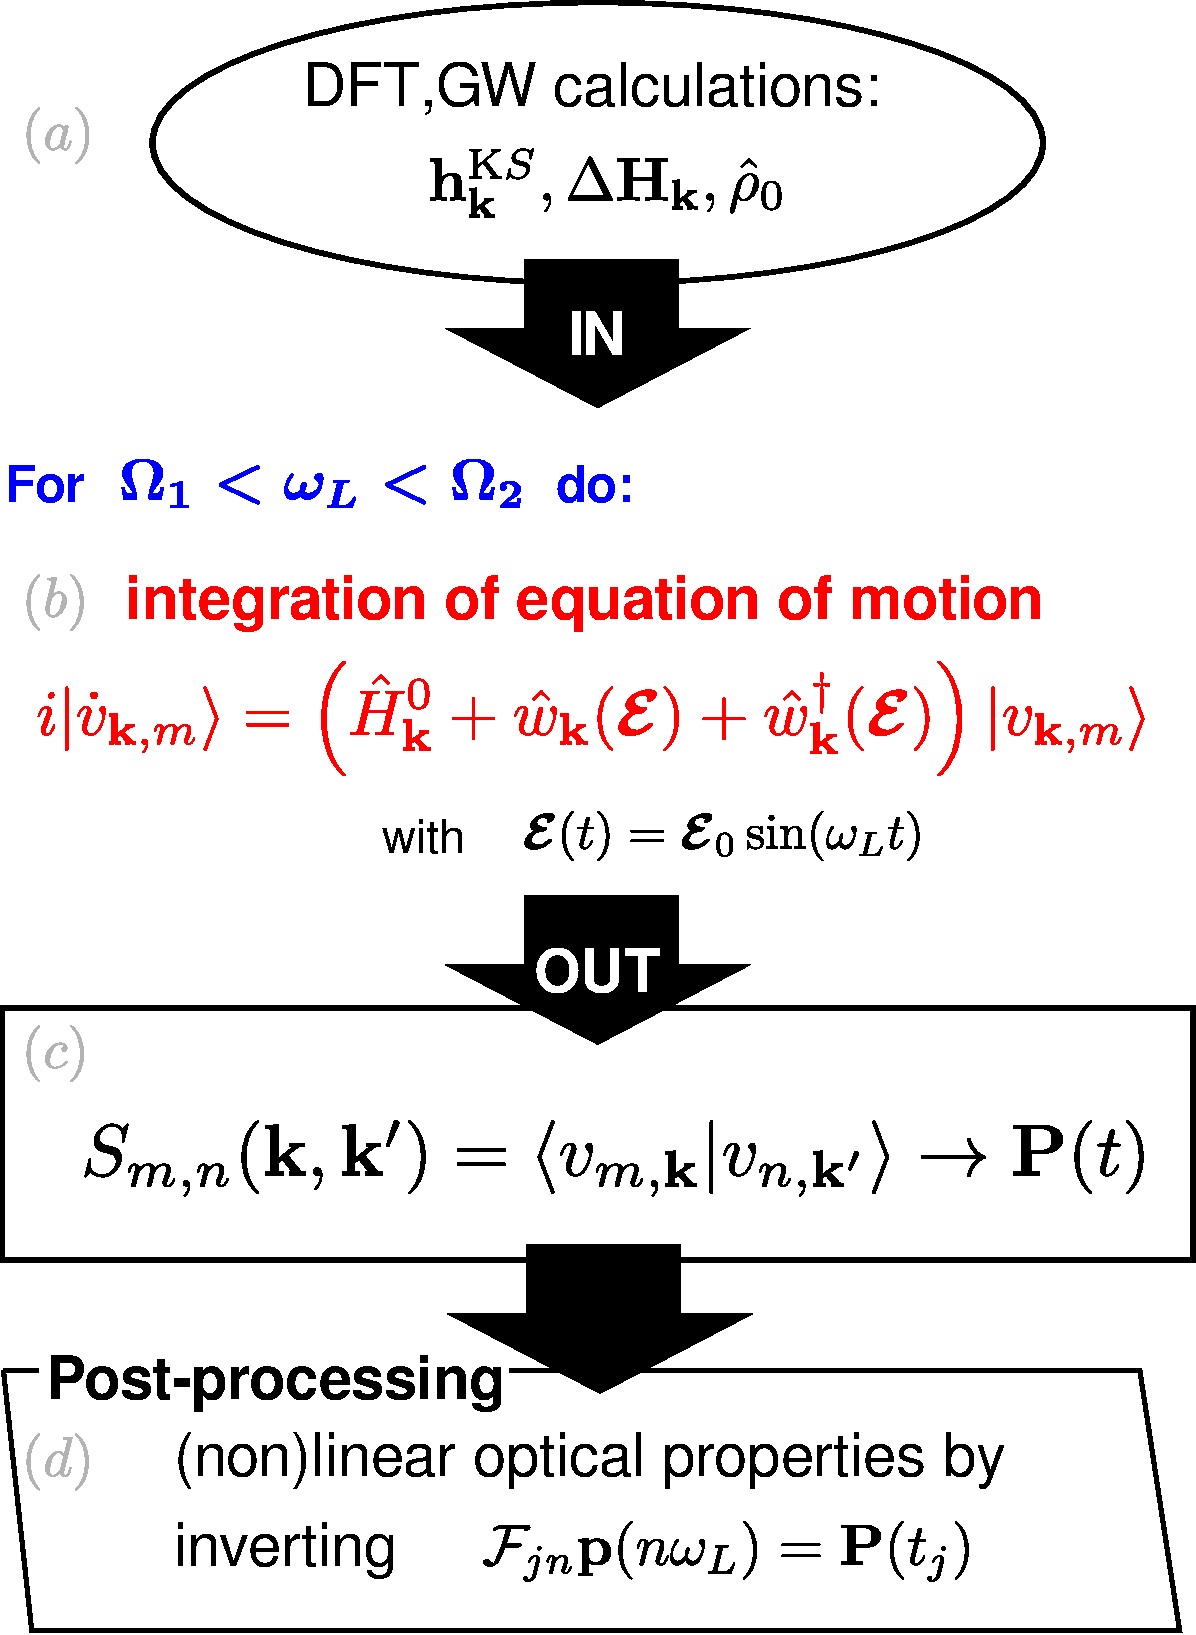
\includegraphics[width=0.4\textwidth]{Figures/scheme-eps-converted-to}
\caption{\footnotesize{Real-time \ai scheme to compute SHG and THG spectra in the $\[\Omega_1,\Omega_2\]$ energy range for extended systems with PBC: $(a)$ Results from KS-DFT and $G_0W_0$ are input to determine the zero-field Hamiltonian. $(b)$ The EOMs [Eq.~\eqref{eom}] are then integrated,  the polarisation is computed as in Eq.~\eqref{berryP2}. In the post-processing step $(d)$ the nonlinear susceptibilities are obtained by inversion of the Fourier matrix [Eq.~\eqref{eq:fouinv}], see Sec.~\ref{sc:compdet} for details.}}
\label{fg:cmpscm}
\end{center}
\end{wrapfigure}

The scheme in Fig.~\ref{fg:cmpscm} has been implemented in the development version of the {\sc Yambo} code.\cite{yambo} 
Kohn-Sham calculations have been performed using the {\sc Abinit} code,\cite{abinit} and the relevant numerical parameters are summarized in Ref.~\cite{nloptics2013}. All the operators  appearing in the EOMs[Eqs.~\eqref{eom},\eqref{eq-tdh},\eqref{eq-tdqpa}] have been expanded in the Kohn-Sham basis set and the number of bands employed in the expansion is again reported in Ref.~\cite{nloptics2013}. 

Rigorously to have a fully \ai scheme, the scissor operator has to be calculated using e.g., $G^0W^0$. In the examples presented in this chapter we use an empirical values for the scissor operator (reported in Ref.~\cite{nloptics2013}) since the scope is to validate the computational scheme, and to facilitate the comparison with other works in the literature.



The EOMs [Eq.~\eqref{eom}] have been integrated using the following algorithm~\cite{koonin90}
\be
\label{eq:time_evolution}
\ket{v_{\kk n}(t+\Delta t)}= \frac{I-i(\Delta t/2)\hat H^0_{\kk}(t)}{I+i(\Delta t/2) \hat H^0_{\kk}(t)} \ket{v_{\kk n}(t)},
\ee
valid for both Hermitian and non-Hermitian Hamiltonians, and strictly unitary for any value of the time-step $\Delta t$ in the Hermitian case. In all real-time simulations we used a time-step of 0.01 fs.\\
%The number of states (number of bands $\times$ number of $\kk$ points) evolved during the simulations is reported in Ref.~\cite{nloptics2013}. \\

\begin{figure}[ht]
\centering
\epsfig{figure=Figures/Pt_analysis.eps,width=8.5cm,clip}
\caption{\footnotesize{Pictorial representation of the signal analysis in the post-processing step. The signal  $P(t)$ (red line) can be divided into two regions: an initial convergence region (up to $t\gg 1/\gamma_{deph}$) in which the eigenfrequencies of the systems are ``filtered out'' by dephasing and a second region where Eq.~\eqref{eq:frrexp} holds. In this second region the signal $P(t)$ is sampled within a period $T_L=2\pi/\omega_L$ to extract the $P^\alpha_i$ coefficients of Eq.~\ref{eq:fouinv}. Note that $P(t)$ is not a realistic one: for illustration purposes we enhanced the second-harmonic signal that otherwise would not be visible on this scale.}} 
\label{fg:ptanalysis}
\end{figure} 

In our simulations we switch on the monochromatic field at $t=t_0$. This sudden switch excites the eigenfrequencies of the system $\omega^{0}_l$ introducing spurious contributions to the non-linear response.
We thus add an imaginary term into the Hamiltonian $H^{0}_\kk$ to simulate a finite dephasing:   
\be
\Gamma= -\frac{i}{\gamma_{\text{deph}}} \sum_l  \{  | v_{\kk,l}\rangle \langle  v_{\kk,l} | - | v^0_{\kk,l}\rangle \langle  v^0_{\kk,l} | \}
\label{dethterm}
\ee
where $|v^0_{\kk,l}\rangle$ are the valence bands of the unperturbed system and $\gamma_{\text{deph}}$ is the dephasing rate. Then we run the simulations for a time much larger than $1/\gamma_{\text{deph}}$ and sample $\PP(t)$ close to the end of the simulation, see Figure~\ref{fg:ptanalysis}.
Since $\gamma_{\text{deph}}$ determines also the spectral broadening, we cannot choose it arbitrary small. For example in the present calculations we have chosen $1/\gamma_{\text{deph}}$ equal to 6 fs that corresponds to a broadening of approximately 0.2 eV (comparable with the experimental one) and thus we run the simulations for 50-55 fs.\\
Once all the eigenfrequencies of the system are filtered out, the remaining polarisation $\PP(t)$ is a periodic function of period $T_L =\frac{2\pi}{\omega_L}$, where $\omega_L$ is the frequency of the external perturbation and can be expanded in a Fourier series
\be\label{eq:frrexp}
\PP(t) = \sum_{n=-\infty}^{+\infty} \pp_n e^{-i\omega_n t},
\ee  
with $\omega_n = n \omega_L$, and complex coefficients:
\begin{equation}\label{eq:frrcff}
 \pp_n = F\{\PP(\omega_n)\} =\int_{0}^{T_L} dt \PP(t) e^{i\omega_n t}.
\end{equation}
To obtain the optical susceptibilities of order $n$ at frequency $\omega_L$ one needs to calculate the $\pp_n$ of Eq.~\eqref{eq:frrexp}, proportional to $\susc n$ by the $n$-th power of the $\efield_0$. 
However, the expression in Eq.~\eqref{eq:frrcff} is not the most computationally convenient since one needs a very short time step---significantly shorter than the one needed to integrate the EOMs---to perform the integration with sufficient accuracy. As an alternative we use directly Eq.~\eqref{eq:frrexp}: we truncate the Fourier series to an order $S$ larger than the one of the response function we are interested in. We sample $2S+1$ values $\PP_i\equiv\PP(t_i)$ within a period $T_L$, as illustrated in Figure~\ref{fg:ptanalysis}. Then Eq.~\eqref{eq:frrexp} reads as a system of linear equations 
\be
{\cal F}_{in} p^\alpha_n = P^\alpha_i,
\label{eq:fouinv}
\ee 
from which the component $p^\alpha_n$ of $\pp_n$ in the $\alpha$ direction is found by inversion of the $(2S+1)\times(2S+1)$ Fourier matrix ${\cal F}_{in} \equiv \exp(-i\omega_n t_i)$. We found that the second harmonic generation converges with S equal to 4 while the third harmonic requires S equal to 6. Finally we noticed that averaging averaging the results on more periods can slightly reduce the numerical error in the signal analysis. \\
\begin{figure}[ht]
\centering
\epsfig{figure=Figures/SiC_absX2_QPRPA_vs_Luppi.pdf,width=1\textwidth,clip}
\caption{\footnotesize{Magnitude of $\chi^{(2)}(-2\omega,\omega,\omega)$ for bulk SiC calculated within the IPA (black triangles) and QPA (red circles) $(a)$ panel and RPA (red circles) $(b)$ panel. Each point corresponds to a real-time simulation at the given laser frequency (see Sec.~\ref{sc:compdet}). Comparison is made with results obtained \ai by direct evaluation of the $\chi^{(2)}$ in Ref.~\cite{PhysRevB.82.235201} in IPA (grey solid line) and QPA (brown dashed line) $(a)$  panel and RPA (brown dashed line) $(b)$ panel.  \label{fg:SiCQPRPA} [Figure from Ref.\cite{nloptics2013}]}}
\end{figure}
Alternatively one can opt for a slow switch on of the electric field as in Takimoto et al.,\cite{takimoto:154114} so that no eigenfrequencies of the system are excited, and avoid to introduce imaginary terms in the Hamiltonian. We found, however, that the latter approach also requires long simulations, and on the other hand, it is less straightforward to extract the $\susc n$.


\section{Results}\label{sc:results}
%                                                                                                                     
The main objective of this section is to validate the computational approach described in Secs.~\ref{sc:theory} and \ref{sc:compdet} against results in the literature for SHG obtained by the response theory in frequency domain. In particular we chose to validate against results from Refs.~\cite{PhysRevB.82.235201,PSSB.427.1984} on bulk SiC and AlAs in which the electronic structures is obtained---as in our case---from a pseudo-potential plane-wave implementation of Kohn-Sham DFT with the local density approximation, which makes the comparison easier.
In the following we considered the zinc-blende structure of SiC and AlAs for which the $\susc 2$ tensor has only one independent nonzero component, $\susc 2_{xyz}$ (or its equivalent by permutation).

Figure \ref{fg:SiCQPRPA} show results for the magnitude of SHG in SiC at the IPA, QPA and TDH level of theory. 
At all levels of approximation we obtained an excellent agreement with the results in Ref.~\cite{PhysRevB.82.235201}. The minor discrepancies between the curves are due to the different choice for the $\kk$-grid used for integration in momentum space: we used a $\Gamma$-centred uniform grid (for which we can implement the numerical derivative) whereas Ref.~\cite{PhysRevB.82.235201} used a shifted grid. Figure~\ref{fg:AlAsQPRPA} shows results for the magnitude of SHG in AlAs at the IPA, QPA and TDH level of theory. 
Also in this case results obtained from our real-time simulations agree very well with the reference results and again the small differences between the spectra can be ascribed mostly to the different grid for $\kk$-integration.
As side results we can also observe the effects of different levels of approximation for the Hamiltonian on the SHG spectrum. In order to interpret those spectra note that SHG resonances occur when either $\omega_L$ or $2\omega_L$ equals the difference between two single-particle energies. Then one can distinguish two energy region: below the single-particle minimum direct gap where only resonances at $2\omega_L$ can occur, and above where both $\omega_L$ or $2\omega_L$ resonances  can occur.\\
Regarding the quasi-particle corrections to the IPA energy levels by a scissor operator, below the minimum Kohn-Sham direct band gap the IPA spectrum is shifted by half of the value of the scissor shift (0.4 eV for SiC and 0.45 eV for AlAs) and the spectral intensity reduced by a factor 1.18 (SiC) and  1.25 (AlAs). Above the minimum Kohn-Sham direct band gap instead the QPA spectrum cannot be simply obtained by shifting and renormalizing the IPA one because of the occurrence of resonances at $\omega_{L}$, that are shifted and renormalised differently.\\  
Regarding the crystal local field, their global effect is to reduce the intensity with respect to the IPA. For SiC, the intensity is reduced by about 15\% below the gap, while above the band gap TDH and IPA have similar intensities. For AlAs we observe a reduction of about 30\% in intensity for the whole range of considered frequencies, but for frequencies larger than 4 eV (that is where the $\omega_L$ resonances with the main optical transition occur) for which again the TDH and IPA have similar intensities.
\begin{figure}[ht]
\centering
\epsfig{figure=Figures/AlAs_absX2_QPRPA_vs_Luppi.pdf,width=1\textwidth,clip}
\caption{\footnotesize{Magnitude of $\chi^{(2)}(-2\omega,\omega,\omega)$ for bulk AlAs calculated within the IPA (black triangles) and QPA (red circles) $(a)$ panel and RPA (red circles) $(b)$ panel. Each point corresponds to a real-time simulation at the given laser frequency (see Sec.~\ref{sc:compdet}). Comparison is made with results obtained \ai by direct evaluation of the $\chi^{(2)}$ in Refs.~\cite{PhysRevB.82.235201,PSSB.427.1984} in IPA (grey solid and dot-dashed line) and QPA (brown dashed and dotted line) $(a)$ panel and RPA (brown dashed and dotted line) $(b)$ panel. \label{fg:AlAsQPRPA} [Figure from Ref.\cite{nloptics2013}] }}
\end{figure}

\section{Conclusions}\label{conclusion}                                        
In this chapter we presented an \ai real-time approach to calculate nonlinear optical properties of extended systems in the length gauge. The key strengths of the proposed approach are first, the correct treatment of the coupling between electrons and the external field and second the possibility to include easily correlation effects beyond the IPA.

Regarding the treatment of the electron-field coupling, following the work of Souza et al.\cite{souza_prb}, we started from the Berry's phase formulation for the dynamical polarisation---a definition consistent with the periodic boundart conditions (PBC)---to derive a covariant numerical expression for the dipole operator in the EOMs.

Note that we worked in the length-gauge even if the velocity gauge may appear a more natural choice. In fact, as opposed to the position operator the velocity operator is consistent with the PBC. However, in the velocity gauge even if the position operator disappears from the Hamiltonian, it reappears in the phase factor for the wave-function~\cite{PhysRevA.36.2763}, so that the problem of re-defining the position operator remains. 
Furthermore, the velocity gauge is plagued by unphysical numerical divergences for the response at low frequencies~\cite{PhysRevB.52.14636}. 
Concerning effects beyond the independent-particle approximation, they are included by simply adding the corresponding single-particle operator to the Hamiltonian. This is an easy task when compared with deriving the corresponding expressions for the nonlinear optical susceptibility.~\cite{PhysRevB.80.155205,PhysRevB.80.165318} As an example, in the present chapter we have included quasi-particle corrections to the band-gap by adding to the Hamiltonian a scissor operator and crystal local-field effects by adding the time-evolution of the Hartree potential. In principle, one can add as well excitonic effects by adding the time-evolution of the screened exchange self-energy (see chapter~\ref{chaptercorr}); or perform a real-time TD-DFT calculations by adding the time-evolution of the exchange-correlation potential (see chapter~\ref{chaptertddft}). Being the focus of this chapter the validation of the proposed approach for calculating nonlinear properties, the inclusion of these correlation effects is discussed in the rest of this work.
We have proved the validity of our approach by comparing our results, obtained from real-time simulations, with results in the literature obtained from direct evaluation of the second order susceptibility in frequency-domain.  

